
\begin{figure*}
\centering
\begin{subfigure}[b]{0.49\linewidth}
    \centering
    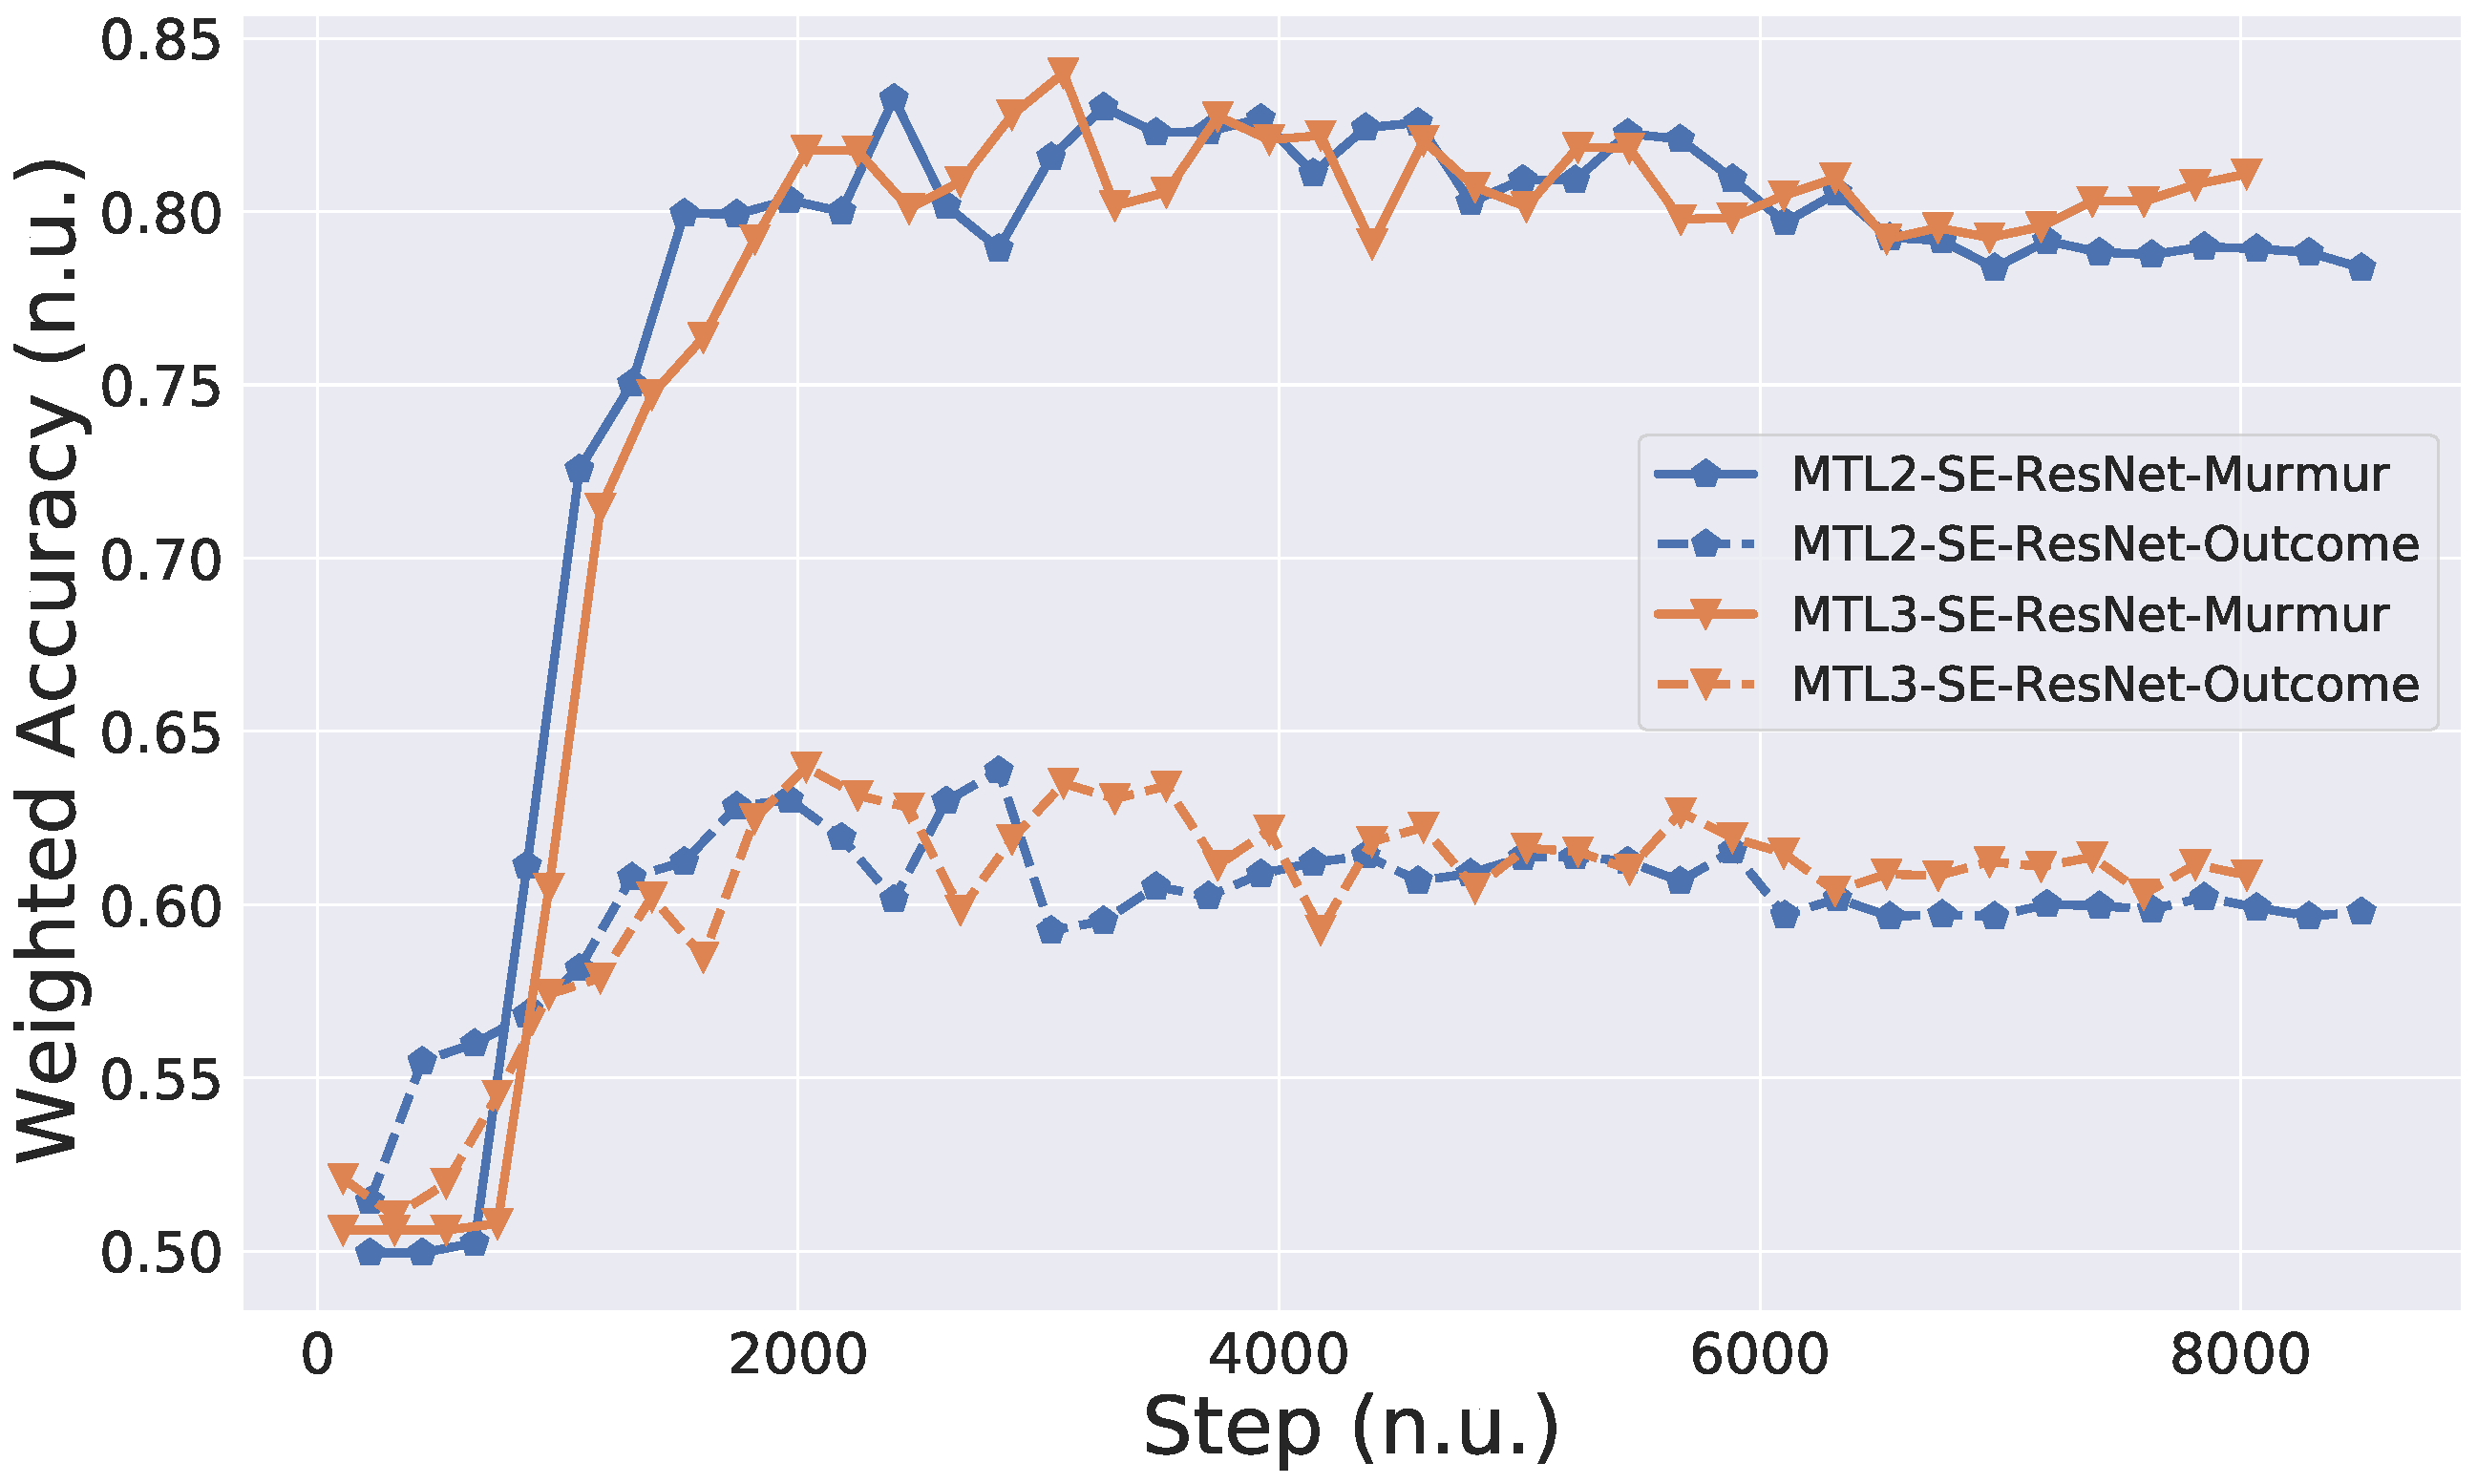
\includegraphics[width=\textwidth]{images/se-resnet-clf-vs-mtl.pdf}
    \caption[]
    {Experiments using SE-ResNet as backbone.}
    \label{fig:se-resnet-clf-vs-mtl}
\end{subfigure}
\hfill
\begin{subfigure}[b]{0.49\linewidth}
    \centering
    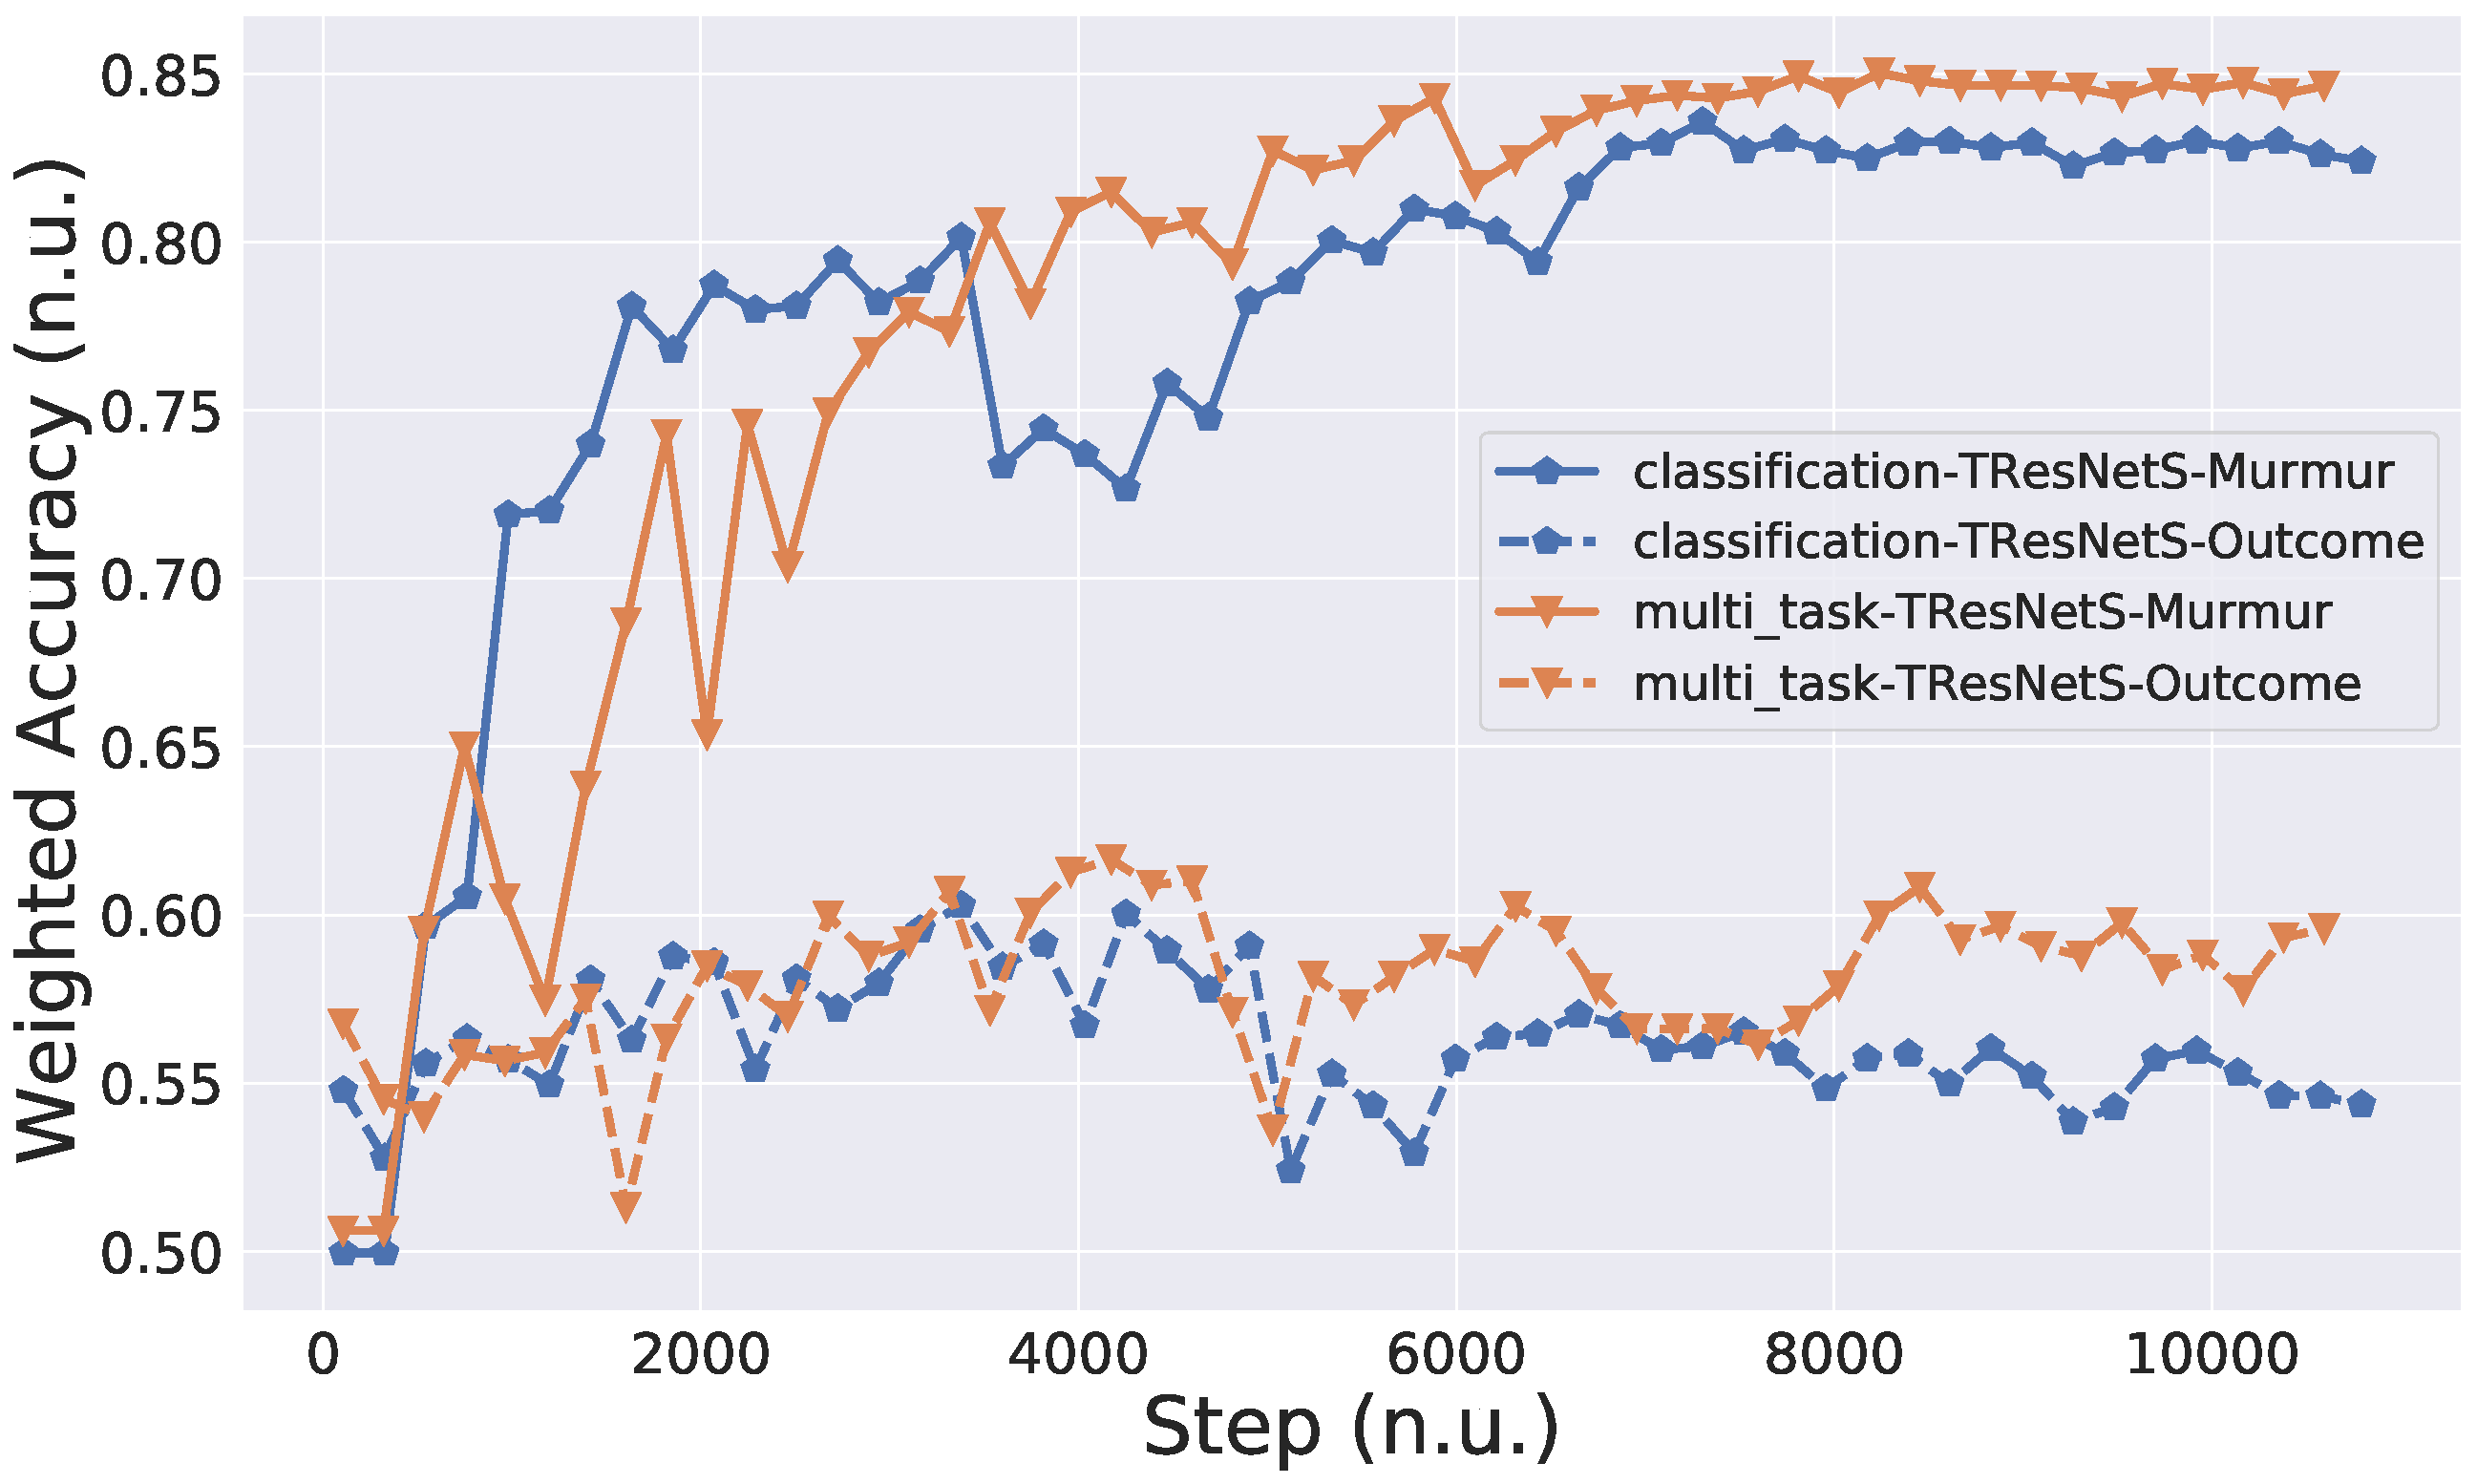
\includegraphics[width=\textwidth]{images/tresnets-clf-vs-mtl.pdf}
    \caption[]
    {Experiments using TResNetS as backbone}
    \label{fig:tresnets-clf-vs-mtl}
\end{subfigure}
\caption[]
{Experiments of the MTL method with 2 heads (for murmur classification and for outcome classification ) and with 3 heads (an additional head for heart sound segmentation) using 2 typical backbones.}
\label{fig:mtl_comparison}
\end{figure*}
